%% This is an example first chapter.  You should put chapter/appendix that you
%% write into a separate file, and add a line \include{yourfilename} to
%% main.tex, where `yourfilename.tex' is the name of the chapter/appendix file.
%% You can process specific files by typing their names in at the 
%% \files=
%% prompt when you run the file main.tex through LaTeX.
\chapter{Conclusions}

With $B^0_s$ and $B^+$ measurements in PbPb collision, we can study beauty hadrochemistry and answer questions 

\section{Comparison with Other Experiments and Theoretical Models}

Because our fully reconstructed B-meson analysis in pp as the reference is still ongoing, in order to understand our PbPb data, we add the B-meson pp measurements from LHCb and ATLAS at different rapidity ranges. Since the rapidity dependence is not significant in $B^0_s/B^+$ ratio as demonstrated in Figure \ref{} from the LHCb publication \ref{}, assuming it is also insignificant in PbPb, we can use the pp reference at different rapidity ranges as references in our $B^0_s/B^+$ measurement

In addition to the pp reference, we also include the prediction from TAMU and Cao, Sun, Ko models, which have been introduced in Section 1.

Figure \ref{FinalResults} show the comparison between our $B^0_s/B^+$ measurement with pp references and theoretical model calculations. 

\begin{figure}[hbtp]
\begin{center}
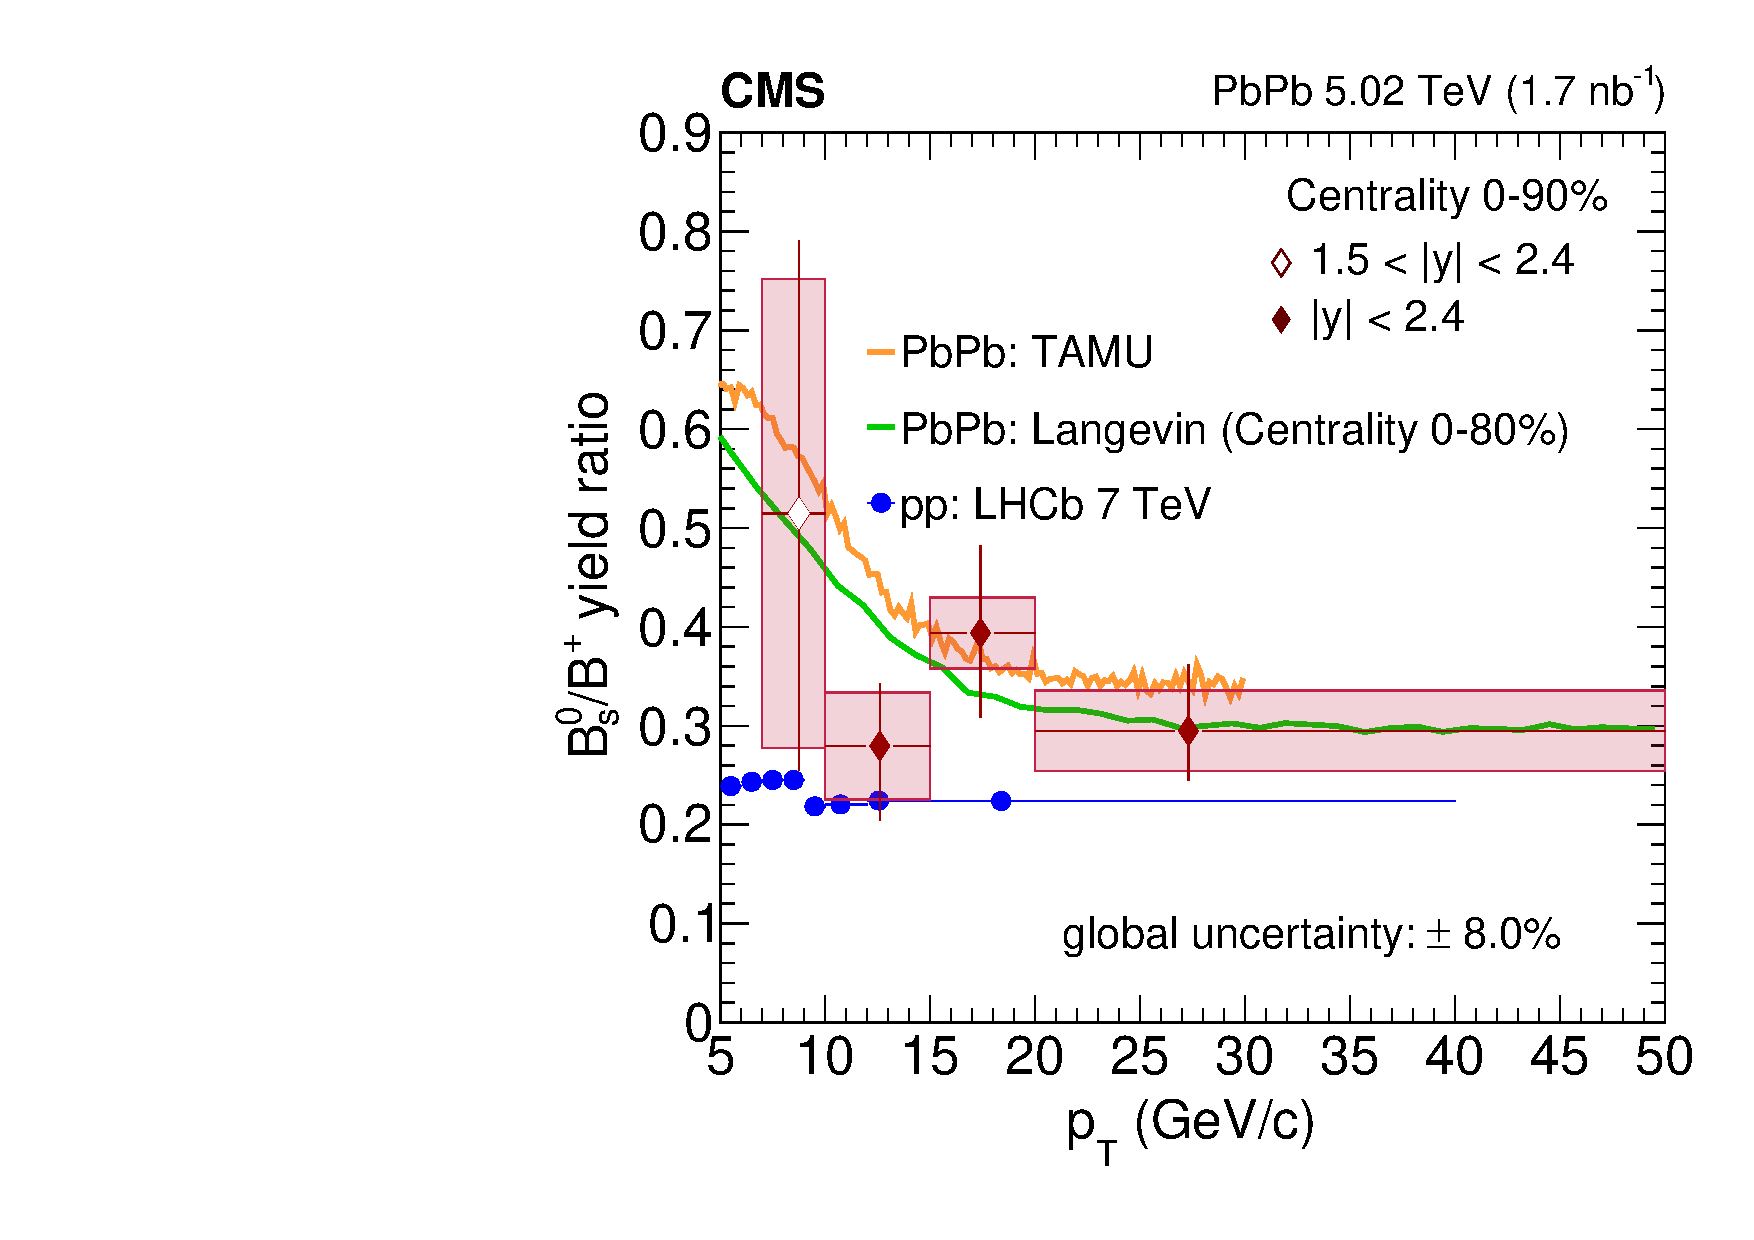
\includegraphics[width=0.48\textwidth]{Figures/Chapter6/ratio_bsbu_vsPt.pdf}
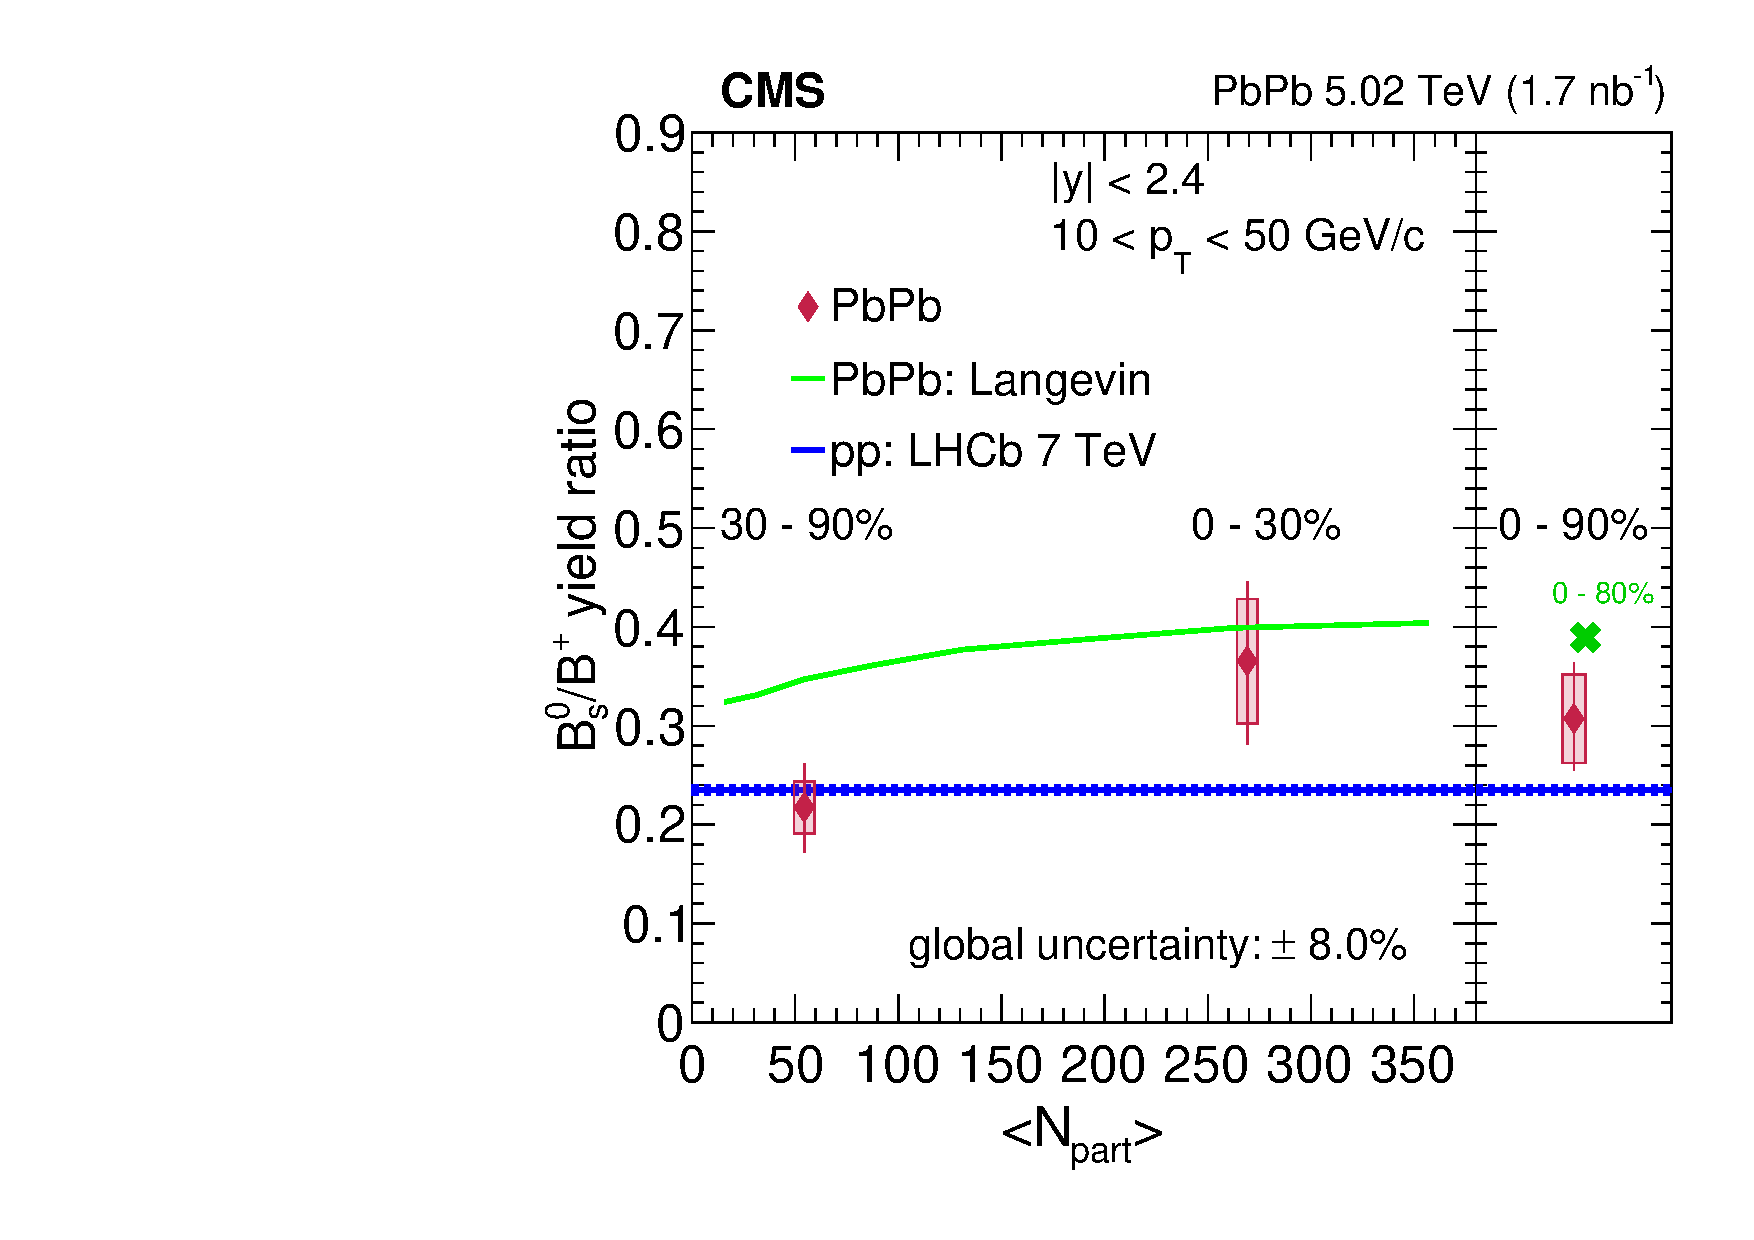
\includegraphics[width=0.48\textwidth]{Figures/Chapter6/ratio_bsbu_vsCent.pdf}
\caption{The fully reconstructed $B^0_s$ and $B^+$ $R_{AA}$ (left) and $B^0_s/B^+$ $R_{AA}$ ratio (right) as a function of $p_T$ using the 2015 CMS pp and PbPb datasets are shown above.}
\label{FinalResults}
\end{center}
\end{figure}   
 

\section{Physics Messages Discussion}

Lies above but with in about 1.5 sigma. not significant $p_T$ dependence. Agree reasonably well with both TAMU and Cao, Sun, Ko models. compatible with LHCb data


\section{Conclusions}

More precise measurement. LHC

\section{Future Outlooks}

As mentioned previous, current results still limited. It would also be great . Figure \ref{} shows our ongoing analysis of fully reconstructed $B^0_s$, $B^+$, and $B^0$ via the decay channels of 


Very clear B-meson signals have been observed. The estimated significance are all greater 4. With these signals, we can perform measurement on $B^+$ cross section in pp collisions down to 0 $p_T$, which allows us to perform measurement of inclusive beauty production cross section. In addition, we will also be able to measure $B^0_s/B^+$ ratio down to 3 GeV/c. Also, according to the multiplicity studies, we can also $B^0_s/B^+$ as a function of multiplicity up to 150, which also help us answer questions raised in Chapter 2. 

Finally, with the sPHENIX experiment at RHIC taking data in 2023, we can also fully reconstruct b hadrons at RHIC energy to study a QGP medium at a lower temperature and higher baryon chemical potential. The beauty measurement at RHIC will be complementary to the measurements at the LHC. Together, these will help determine heavy quark diffusion coefficient with different temperature, constrain the fundamental property of QGP $\eta/s$, and probe the inner workings of QGP. A bright and exciting future of heavy flavor physics in heavy-ion collision will be forthcoming.



